\subsection{UC15 - Sospensione di un alert}
\begin{figure}[H]
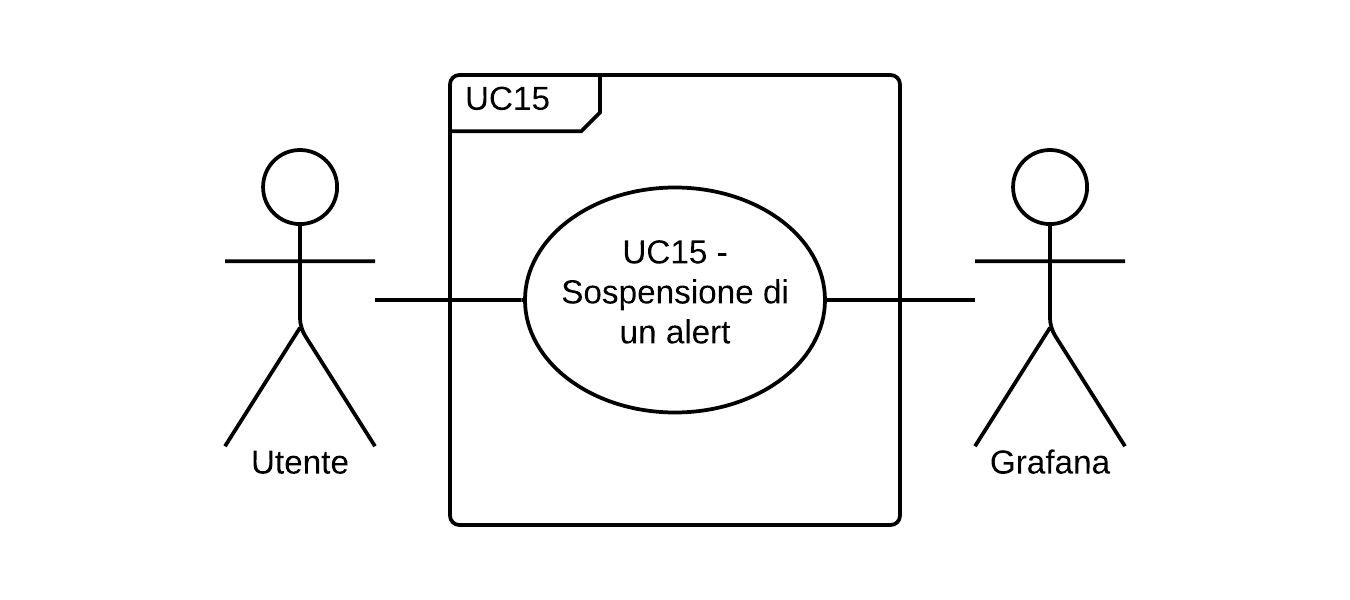
\includegraphics{img/UC15_-_Sospensione_di_un_alert.png}
\caption{Diagramma degli use case di UC15}
\end{figure}
\begin{itemize}
	\item \textbf{Codice identificativo}: UC15;
	\item \textbf{Titolo}: sospensione di un alert\glo;
	\item \textbf{Attore primario}: utente;
	\item \textbf{Attore secondario}: Grafana\glo;
	\item \textbf{Descrizione}: l'utente esegue la sospensione di un alert\glosp, bloccandone temporaneamente l'esecuzione;
	\item \textbf{Precondizione}: l'utente è autenticato nel sistema software Grafana\glosp ed ha aperto il pannello di visualizzazione alert\glo;
	\item \textbf{Postcondizione}: l'alert\glosp selezionato dall'utente è sospeso;
	\item \textbf{Scenario principale}: utilizzando l'apposita funzione offerta da Grafana\glosp l'utente sospende l'esecuzione dell'alert\glosp che ha selezionato.
\end{itemize} 
